% -----------------------------------------------
% Trabalho Final -- Geração Musical Simbólica com Redes Neurais
% Formato ISMIR (template oficial). Compilar com pdfLaTeX + BibTeX (ex.: Overleaf).
% -----------------------------------------------
\documentclass{article}
\usepackage[T1]{fontenc}
\usepackage[utf8]{inputenc}
\usepackage[brazil]{babel}
\usepackage{ismir} % sem a opção "submission": versão com autores identificados
\usepackage{amsmath,amssymb,cite,url}
\usepackage{graphicx}
\usepackage{booktabs}
\usepackage{color}

\title{Corais de Bach com um Transformer Autoregressivo sobre Tokens REMI: \\ Comparação Objetiva com uma Cadeia de Markov}

% ---- Preencha com os dados do grupo (3 a 5 integrantes) ----
\multauthor
  {Integrante 1 \qquad Integrante 2 \qquad Integrante 3 \qquad Integrante 4}
  {Instituição -- Curso / Disciplina\\
   \texttt{\{email1, email2, email3, email4\}@instituicao.br}}
\def\authorname{Integrante 1, Integrante 2, Integrante 3, Integrante 4}

\sloppy

\begin{document}
\maketitle

\begin{abstract}
Treinamos um Transformer autoregressivo, implementado diretamente em PyTorch, para gerar do zero corais a quatro vozes no estilo de J.\,S.~Bach. Os 382 corais do JSB Chorales (partição oficial) são convertidos em MIDI e codificados em tokens REMI (106 tokens). Como \textit{baseline}, uma cadeia de Markov de ordem $n$ com interpolação de Witten--Bell usa os mesmos dados, a mesma representação e o mesmo protocolo de amostragem. O Transformer atinge perplexidade de validação 3{,}00 por token, contra 6{,}38 da melhor cadeia ($n=5$). Em 200 peças por sistema, comparadas às 77 do conjunto de teste com sete métricas do \textit{muspy}, o Transformer reproduz as distribuições humanas de entropia de classes de altura e consistência de escala (área de sobreposição 0{,}92 contra 0{,}20 e 0{,}09 da cadeia). A cadeia deriva entre tonalidades e perde a contagem de vozes. A principal falha restante do Transformer é a textura: só 62\% dos ataques soam com exatamente quatro notas, contra 92\% em Bach.
\end{abstract}

\section{Introdução}\label{sec:intro}
No TP1 geramos corais com cadeias de Markov e observamos o compromisso clássico do método: ordens baixas perdem a estrutura e ordens altas copiam o corpus. Aqui investigamos se um modelo neural autoregressivo, capaz de condicionar a previsão a centenas de eventos passados, supera esse limite.

\textbf{Tarefa.} \emph{Composição livre incondicional}: a partir apenas de um token de início (BOS), gerar um coral completo a quatro vozes (soprano, contralto, tenor e baixo), em compasso quaternário, até o token de fim (EOS). Não há condicionamento nem trecho inicial. A comparação é com as peças humanas do conjunto de teste, por métricas objetivas de distribuição~\cite{yang2020evaluation}.

Entregamos um \textit{pipeline} reprodutível (dados, tokens, treino, geração, avaliação e áudio), uma cadeia de Markov comparável ao Transformer em verossimilhança e em amostras, e uma análise de onde cada modelo falha.

\section{Trabalhos Relacionados}\label{sec:related}
\textbf{Corais de Bach.} O JSB Chorales foi popularizado por Boulanger-Lewandowski et al.~\cite{boulanger2012} como \textit{benchmark} de modelagem polifônica. Allan e Williams~\cite{allan2005} harmonizam melodias com HMMs. O BachBot~\cite{liang2017bachbot} gera corais com LSTMs sobre uma sequência que intercala as vozes. O DeepBach~\cite{hadjeres2017} usa redes recorrentes bidirecionais com amostragem de Gibbs para permitir restrições. O Coconet~\cite{huang2017coconet} trata a geração como preenchimento de uma grade com uma rede convolucional e disponibiliza a versão em semicolcheias do dataset que usamos.

\textbf{Transformers e representações.} O Transformer~\cite{vaswani2017} foi levado à música pelo Music Transformer~\cite{huang2019musictransformer}, sobre eventos MIDI-Like~\cite{oore2020}. O REMI~\cite{huang2020remi} troca os deslocamentos temporais por tokens de compasso e posição na grade métrica. O Compound Word~\cite{hsiao2021cp} agrupa os atributos de uma nota num único passo. Usamos a implementação do REMI do \textit{miditok}~\cite{fradet2021miditok}.

\textbf{Markov e avaliação.} Cadeias de Markov são a técnica mais antiga de composição algorítmica~\cite{hiller1959,ames1989,conklin2003}; em ordem alta, plagiam o corpus~\cite{papadopoulos2014}. Para avaliar, seguimos Yang e Lerch~\cite{yang2020evaluation}, que comparam distribuições de métricas em vez de médias, e calculamos as métricas com o \textit{muspy}~\cite{dong2020muspy}.

\section{Método}\label{sec:method}
\textbf{Dataset e pré-processamento.} Usamos o JSB Chorales~\cite{boulanger2012} na versão de Huang et al.~\cite{huang2017coconet}, com a partição oficial de 229, 76 e 77 corais (treino, validação e teste). A separação é por peça, e o teste só foi usado na avaliação final. Cada coral é uma grade em semicolcheias com as quatro alturas por passo. Passos consecutivos de mesma altura numa voz viram uma nota sustentada (o formato não distingue nota repetida de ligadura). Como o arquivo não traz compasso nem anacruse, tratamos todos os corais como 4/4 e prefixamos $(16 - T \bmod 16) \bmod 16$ passos de silêncio, para que o último compasso termine na barra. As notas viram um MIDI de faixa única (órgão, 80\,bpm). No treino aplicamos aumento de dados por transposição em $-5,\dots,+6$ semitons, descartando cópias fora da tessitura do vocabulário (Lá1--Ré6). Assim, 229 corais viram 2706 sequências (1{,}44\,M tokens). Em média, um coral tem 15{,}1 compassos e 215 notas, com alturas MIDI de 36 a 81.

\textbf{Representação.} Usamos REMI~\cite{huang2020remi} via \textit{miditok}~\cite{fradet2021miditok}, com as quatro vozes fundidas numa única sequência. Cada nota é codificada como \texttt{Pitch}+\texttt{Duration}; cada instante de ataque, como \texttt{Position} (16 por compasso); e cada compasso, como \texttt{Bar}. Desativamos velocidade, andamento, acordes e programas, que o corpus não contém, e os tokens de bateria que o \textit{miditok} inclui por padrão. As durações têm resolução de semicolcheia até um compasso e de colcheia até três compassos. O vocabulário final tem \textbf{106 tokens}: 54 alturas, 32 durações, 16 posições, \texttt{Bar}, PAD, BOS e EOS. O comprimento médio é de 535$\pm$174 tokens por coral no treino (522 na validação e 566 no teste; máximo de 1823). Do total, 40\% são \texttt{Pitch}, 40\% \texttt{Duration}, 16\% \texttt{Position} e 3\% \texttt{Bar}. Escolhemos o REMI porque a grade métrica explícita casa com a escrita homorrítmica dos corais, em que quase todo tempo é um ataque de acorde: a posição no compasso é um símbolo previsto pelo modelo, e não algo a acumular a partir de deslocamentos temporais, como no MIDI-Like.

\textbf{Modelo.} Usamos um Transformer \textit{decoder-only}: embedding de tokens somado a um embedding posicional aprendido (contexto de 1024), quatro \texttt{nn.TransformerEncoderLayer} com pré-normalização, $d=256$, 4~cabeças, \textit{feed-forward} de 1024 com GELU e máscara causal, seguidos de uma camada de normalização e de uma projeção de saída com pesos amarrados ao embedding. São 3{,}45\,M parâmetros. A classe do modelo, o laço de treino e a amostragem foram escritos pelo grupo em PyTorch~\cite{paszke2019}, sem bibliotecas de alto nível. Um teste unitário verifica que mudar tokens futuros não altera as saídas passadas, tanto no modo de treino quanto no de inferência.

\textbf{Baseline.} Usamos uma cadeia de Markov de ordem $n$ sobre os \emph{mesmos} tokens e as mesmas 2706 sequências de treino. Diferentemente do TP1, cuja cadeia só define probabilidades para contextos vistos (com \textit{back-off}), interpolamos todas as ordens com o método de Witten--Bell~\cite{witten1991}:
\begin{equation}
P_k(w\mid h_k)=\frac{c(h_k,w)+T(h_k)\,P_{k-1}(w\mid h_{k-1})}{c(h_k)+T(h_k)},
\end{equation}
em que $T(h)$ é o número de tokens distintos já vistos após o contexto $h$ e $P_0$ é o unigrama com suavização de Laplace. Isso dá uma distribuição própria sobre os 106 tokens em qualquer contexto, o que permite calcular a perplexidade e aplicar o mesmo amostrador do Transformer. A ordem $n\in\{0,\dots,16\}$ é escolhida pela NLL de validação.

\textbf{Amostragem.} Os dois sistemas usam a mesma função: temperatura $T=1$, núcleo top-$p=0{,}95$~\cite{holtzman2020}, PAD e BOS proibidos, parada em EOS ou em 2600 tokens. No Transformer, o contexto desliza quando a sequência passa de 1024 tokens. Os tokens gerados são decodificados pelo \textit{miditok}, e uma gramática simples do REMI mede a taxa de erros sintáticos (por exemplo, \texttt{Pitch} sem \texttt{Duration}).

\section{Experimentos}\label{sec:exp}
\textbf{Configuração.} Treinamos com AdamW~\cite{loshchilov2019} ($\beta=(0{,}9;\,0{,}98)$, \textit{weight decay} 0{,}05), taxa de aprendizado de $5\cdot10^{-4}$ com 500 passos de aquecimento e decaimento cosseno até 10\%, lotes de 16 sequências (recorte aleatório de 1025 tokens quando necessário), \textit{clipping} de gradiente em 1{,}0, precisão bf16 e até 60 épocas, com parada antecipada (paciência de 8) pela NLL de validação. O único hiperparâmetro ajustado foi o \textit{dropout}, entre $\{0{,}15;\,0{,}3\}$, também pela validação. Hardware: uma GPU RTX 3060 Laptop (6\,GB); o treino escolhido levou 11{,}5\,min. A cadeia é ajustada em 22\,s na CPU.

\textbf{Métricas e protocolo.} Cada sistema gera 200 peças com semente fixa, e a referência são os 77 corais de teste, passados pelo mesmo tokenizador. Usamos sete métricas do \textit{muspy}~\cite{dong2020muspy}: extensão, número de classes de altura usadas, entropia de classes de altura, consistência de escala (maior fração de notas dentro de uma escala maior ou menor), polifonia (média de alturas simultâneas), taxa de tempos vazios e consistência de \textit{groove}. Acrescentamos o número de compassos. Para cada métrica, seguimos Yang e Lerch~\cite{yang2020evaluation}: estimamos por KDE a distribuição das distâncias intra-conjunto do teste ($|x_i-x_j|$) e a das distâncias inter-conjuntos gerado--teste. Reportamos a área de sobreposição (OA, quanto maior melhor) e a divergência KL(intra$\|$inter) (quanto menor melhor). Também medimos a NLL de validação de ambos os modelos e fazemos uma análise tonal simples (Krumhansl--Schmuckler) da abertura e do final das peças.

\section{Resultados e Discussão}\label{sec:results}
\begin{figure}[t]
\centering
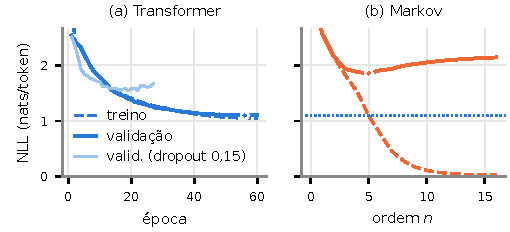
\includegraphics[width=\columnwidth]{figures/training.pdf}
\caption{(a)~NLL por token do Transformer (dropout 0{,}3) por época; a curva clara é a validação com dropout 0{,}15, que sobreajusta a partir da época 19. (b)~NLL da cadeia de Markov por ordem $n$; a linha pontilhada é a melhor NLL de validação do Transformer.}
\label{fig:training}
\end{figure}

\textbf{Verossimilhança.} O Transformer escolhido (dropout 0{,}3, melhor época 56) atinge NLL de validação de 1{,}098 nats/token (perplexidade 3{,}00), contra 1{,}853 (6{,}38) da melhor cadeia, de ordem $n=5$ (Fig.~\ref{fig:training}). Com dropout 0{,}15, o modelo sobreajusta cedo: NLL de treino de 0{,}68 e de validação de 1{,}54. Na cadeia, a NLL de treino cai a quase zero com $n\ge10$ (contextos longos praticamente determinísticos), enquanto a de validação piora: a cadeia passa a copiar o treino, o mesmo fenômeno observado no TP1. Para $n=5$ já há 287\,mil contextos distintos.

\begin{table*}[t]
\centering\small
\setlength{\tabcolsep}{4pt}
\begin{tabular}{@{}lccccccc@{}}
\toprule
 & Teste (humano) & \multicolumn{3}{c}{Transformer} & \multicolumn{3}{c}{Markov ($n=5$)} \\
\cmidrule(lr){2-2}\cmidrule(lr){3-5}\cmidrule(l){6-8}
Métrica & $\mu\pm\sigma$ & $\mu\pm\sigma$ & OA$\uparrow$ & KL$\downarrow$ & $\mu\pm\sigma$ & OA$\uparrow$ & KL$\downarrow$ \\
\midrule
Extensão (semitons)           & 34{,}35$\pm$2{,}73 & 36{,}03$\pm$3{,}20 & \textbf{0{,}94} & \textbf{0{,}033} & 39{,}03$\pm$6{,}18 & 0{,}60 & 0{,}476 \\
Classes de altura usadas      & 10{,}55$\pm$1{,}10 & 10{,}98$\pm$0{,}94 & 0{,}84 & 0{,}131 & 11{,}40$\pm$1{,}61 & \textbf{0{,}90} & \textbf{0{,}055} \\
Entropia de classes de altura & 3{,}03$\pm$0{,}10 & 3{,}03$\pm$0{,}08 & \textbf{0{,}92} & \textbf{0{,}030} & 3{,}40$\pm$0{,}34 & 0{,}20 & 1{,}843 \\
Consistência de escala        & 0{,}930$\pm$0{,}035 & 0{,}930$\pm$0{,}028 & \textbf{0{,}92} & \textbf{0{,}029} & 0{,}688$\pm$0{,}080 & 0{,}09 & 2{,}828 \\
Polifonia                     & 3{,}92$\pm$0{,}04 & 3{,}80$\pm$0{,}11 & \textbf{0{,}44} & \textbf{0{,}878} & 4{,}29$\pm$1{,}00 & 0{,}15 & 2{,}343 \\
Taxa de tempos vazios         & 0{,}035$\pm$0{,}026 & 0{,}040$\pm$0{,}026 & \textbf{0{,}96} & \textbf{0{,}018} & 0{,}082$\pm$0{,}069 & 0{,}68 & 0{,}364 \\
Consistência de \textit{groove} & 0{,}998$\pm$0{,}000 & 0{,}999$\pm$0{,}000 & \textbf{0{,}93} & \textbf{0{,}018} & 0{,}998$\pm$0{,}000 & \textbf{0{,}93} & 0{,}032 \\
Nº de compassos               & 15{,}9$\pm$6{,}0 & 15{,}5$\pm$5{,}7 & \textbf{0{,}95} & \textbf{0{,}021} & 13{,}1$\pm$11{,}6 & 0{,}68 & 0{,}256 \\
\midrule
Ataques com exatamente 4 notas & 92\% & \multicolumn{3}{c}{62\%} & \multicolumn{3}{c}{18\%} \\
Abre e fecha no mesmo tom (K--S) & 52\% & \multicolumn{3}{c}{46\%} & \multicolumn{3}{c}{37\%} \\
Baixo final na tônica da abertura & 69\% & \multicolumn{3}{c}{36\%} & \multicolumn{3}{c}{23\%} \\
\bottomrule
\end{tabular}
\caption{Métricas objetivas: 77 corais de teste contra 200 peças por sistema. OA e KL comparam a distribuição de distâncias intra-teste com a de distâncias gerado--teste~\cite{yang2020evaluation}. As três últimas linhas vêm da nossa análise tonal (Krumhansl--Schmuckler nos 4 primeiros e nos 4 últimos compassos). Nenhum sistema gerou erros sintáticos de REMI.}
\label{tab:metrics}
\end{table*}

\begin{figure*}[t]
\centering
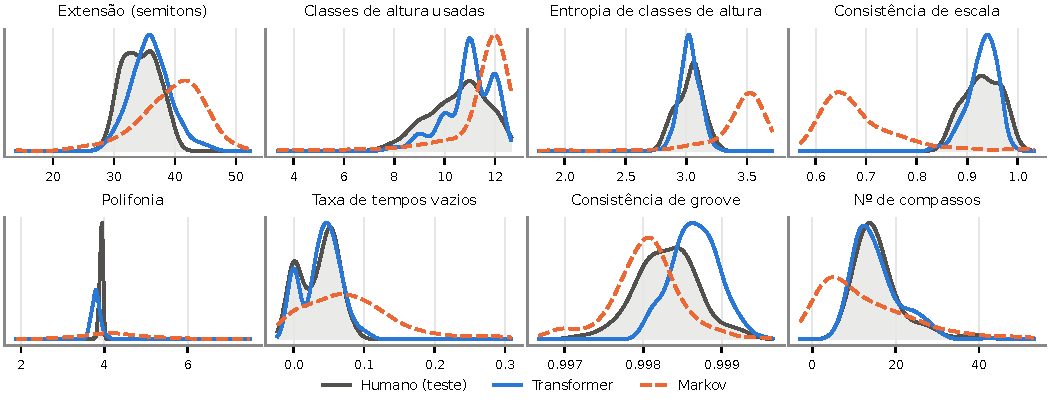
\includegraphics[width=\textwidth]{figures/metrics.pdf}
\caption{Distribuições (KDE) de cada métrica por peça: teste (área cinza), Transformer e Markov.}
\label{fig:metrics}
\end{figure*}

\textbf{Métricas objetivas.} A Tabela~\ref{tab:metrics} e a Fig.~\ref{fig:metrics} mostram que o Transformer tem OA maior ou igual e KL menor que a cadeia em sete das oito métricas. As diferenças decisivas são tonais: a entropia de classes de altura e a consistência de escala do Transformer coincidem com as de Bach (0{,}930 nos dois casos; OA de 0{,}92), enquanto a cadeia usa quase todas as 12 classes de altura de modo uniforme (entropia de 3{,}40 contra 3{,}03; consistência de 0{,}69). Como cada ataque ocupa em média seis tokens (um \texttt{Position} e até quatro pares \texttt{Pitch}+\texttt{Duration}), o contexto de $n=5$ tokens não cobre sequer um ataque completo, e a cadeia não tem como lembrar a tonalidade e modula a cada poucos tempos. Ela também não sabe quantas notas já emitiu num ataque: sua polifonia tem desvio-padrão de 1{,}0, contra 0{,}04 no teste, e só 18\% dos seus ataques têm quatro notas. A única métrica em que a cadeia vence é o número de classes de altura usadas, porque o próprio Bach usa de 10 a 12 classes por coral (modulações e cromatismos de passagem); o Transformer concentra-se mais em 11--12. A consistência de \textit{groove} ($\approx$0{,}998 em todos os conjuntos) não discrimina sistemas homorrítmicos. O número de compassos do Transformer acompanha o do teste, ou seja, ele aprendeu quando emitir EOS; a cadeia gera muitas peças curtas e algumas longas demais.

\textbf{Limitações do Transformer.} A polifonia é a métrica em que ele mais se afasta do teste (OA de 0{,}44): a média de 3{,}80 vozes está abaixo das 3{,}92 de Bach, e só 62\% dos ataques soam com exatamente quatro notas. Como a representação funde as vozes, nada impede o modelo de omitir ou duplicar uma nota no mesmo ataque. Em termos de forma, só 36\% das peças terminam com o baixo na tônica da tonalidade de abertura (69\% no teste): o modelo gera frases tonais coerentes, mas o arco global, que começa e termina no mesmo tom, ainda é fraco.

\textbf{Análise qualitativa.} As peças de demonstração são as cinco primeiras amostras de avaliação de cada sistema, sem escolha a dedo; os MIDI e os áudios estão no repositório (\url{https://github.com/USUARIO/REPOSITORIO}, pasta \texttt{samples/}). Inspecionamos as partituras acorde a acorde. Em \textit{transformer\_004} (Lá$\flat$ maior, 14 compassos) há um acorde por tempo, com o baixo alternando entre tônica, dominante e subdominante, e o final é uma cadência perfeita (Si$\flat$--Mi$\flat$--Lá$\flat$) com o acorde de tônica sustentado por um compasso, como numa fermata. \textit{transformer\_001} (Mi maior) mantém a tonalidade, mas termina no IV grau (Lá maior), um final suspenso. Nas cinco peças, de 31\% a 57\% dos ataques não têm exatamente quatro notas (há uníssonos entre vozes e vozes omitidas), o que é coerente com a métrica de polifonia. As peças da cadeia alternam ataques de duas notas com aglomerados de 11 a 17 notas simultâneas (o máximo de cada peça) e tempos de silêncio no meio da frase, e a estimativa de tonalidade muda entre a abertura e o final nas cinco (ex.: \textit{markov\_001}: Dó menor $\to$ Dó$\sharp$ menor). A cadeia reproduz a gramática local do REMI (nenhum erro sintático), mas não a música.

\section{Conclusão e Trabalhos Futuros}\label{sec:conclusion}
Um Transformer pequeno (3{,}45\,M parâmetros), treinado em 11 minutos sobre 229 corais transpostos, gera corais cujas distribuições de tonalidade e de comprimento ficam muito próximas das de Bach, e reduz a perplexidade de validação a menos da metade da obtida pela melhor cadeia de Markov sobre a mesma representação. A cadeia falha por falta de contexto: o que no TP1 era um compromisso entre estrutura e plágio vira, sobre tokens REMI, incapacidade de manter a tonalidade e o número de vozes.

\textbf{Limitações.} (i)~A textura a quatro vozes não é garantida pela representação. (ii)~Todos os corais são tratados como 4/4, e a anacruse é inferida. (iii)~O dataset não distingue nota repetida de nota ligada. (iv)~Usamos uma única semente por configuração; uma execução anterior com a mesma configuração e um vocabulário maior (com tokens de bateria nunca usados) parou com NLL de 1{,}49, o que indica variância considerável entre execuções. (v)~Não há avaliação perceptiva: a análise qualitativa se baseou na inspeção das partituras.

\textbf{Trabalhos futuros.} Tokens de voz (ex.: o \texttt{Program} do REMI, ou uma voz por posição, como no BachBot~\cite{liang2017bachbot}) para impor as quatro vozes; tokens de compasso e de tonalidade como condição; agrupamento das notas por ataque, como no Compound Word~\cite{hsiao2021cp}; e um teste de audição com participantes.

\bibliography{refs}

\end{document}
